% 实验二分析与讨论
\subsection{实验现象原理分析}

\subsubsection{积分特性与 $\Lambda$-集合}
在对 AES 的积分攻击中，我们构造一个特殊的明文集合，称为 $\Lambda$-集合。在该集合中，选定的字节遍历 $0 \dots 255$（称为 Active 字节），而其余字节保持固定（称为 Constant 字节）。\cite{WongBlock,ZhihuAES}\
\footnote{参考文献2的链接目前已失效(或许是作者没有维护)，但是可以通过互联网档案馆（Wayback Machine）访问：\url{https://web.archive.org/web/20240101000000*/https://www.davidwong.fr/blockbreakers/index.html}。}

设活跃字节遍历的256个取值为 $x_i(i=1,2,\ldots,256)$，满足
\[
\bigoplus_{i=1}^{256} x_{i} = 0
\]
这种性质可以称为\textbf{平衡性}

下面给出证明

有限域\(GF(2^n)\)可以被看作是定义在\(GF(2)\)上的 \(n\) 维向量空间。
这意味着域中的元素可以看作长度为 \(n\) 的二进制向量，
考虑这\(2^n\)个向量在第 \(i\) 位上的取值。
在所有可能的\(2^n\)个组合中，第 \(i\) 位为 0 的元素个数和为 1 的元素个数是相等的。
具体来说，各有\(2^{n-1}\)个。因而有偶数个 1 在第  \(i\) 位进行异或，结果必然是 0。

实验表明，对于一个包含 256 个明文的 $\Lambda$-集合，在经过 3 轮 AES 加密后，其密文状态满足：
\begin{equation}
    \bigoplus_{i=1}^{256} C^{(i)} = 0
\end{equation}

下面展开具体说明
\subsubsection{AddRoundKey不影响活跃字节}
\begin{figure}[H]
    \centering
    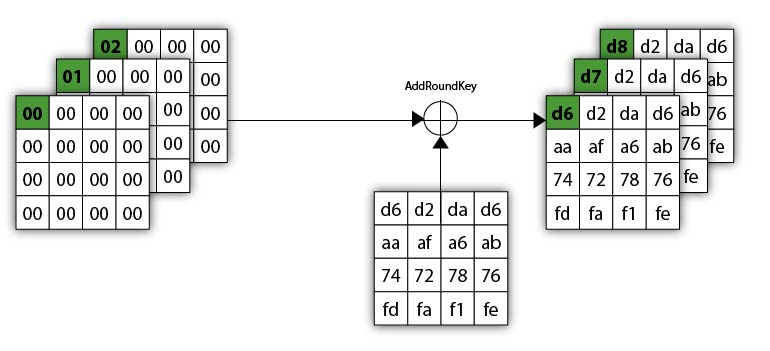
\includegraphics[width=0.8\textwidth]{figure/SQUARE-03.jpg}
\end{figure}
首先一开始先将明文和密钥进行 AddRoundKey 操作，之后进入第 1 轮。异或是线性运算，当活跃字节遍历 $0 \dots 255$ 时，输出字节也会完整遍历 $0 \dots 255$。所以AddRoundKey操作不影响活跃性。
\footnote{实验中要求的活跃字节在矩阵坐标 $(1,0)$ 处的字节，即第二行第一列的字节。此处引用的参考文献中活跃字节在位置(0,0)(如图片所示),此处引用文献图片为方便说明,实际原理相同。} % 但是由于参考文献2的图片绘制精美，此处我想直接使用该文献中的图片来说明AddRoundKey不影响活跃字节的原因。}
\subsubsection{SubBytes不影响活跃字节}
\begin{figure}[H]
    \centering
    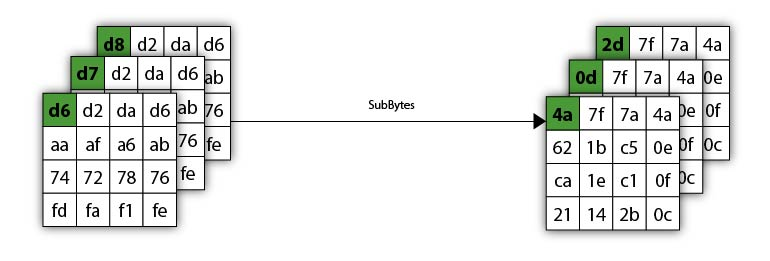
\includegraphics[width=0.8\textwidth]{figure/SQUARE-04.jpg}
\end{figure}
SubBytes(过S盒,字节代换) 是一个\(\{0,1\}^8 \to \{0,1\}^8\) 的映射。因此，活跃字节在经过 SubBytes 后仍然保持活跃，继续遍历 $0 \dots 255$。
\subsubsection{ShiftRows不影响活跃字节数量，但是可能影响活跃字节的位置}
ShiftRows 只是对状态矩阵的行进行循环移位，不改变字节的值。因此，活跃字节在经过 ShiftRows 后仍然保持活跃。
由于第一行不进行移位，所以文献中并未改变活跃字节位置。但是对于实验中的位置，活跃字节在 $(1,0)$ 的情况，经过 ShiftRows 后它会移动到 $(1,3)$，但仍然是活跃的,只是换了一个位置。
\subsubsection{列混淆（MixColumns）的作用}
\begin{figure}[H]
    \centering
    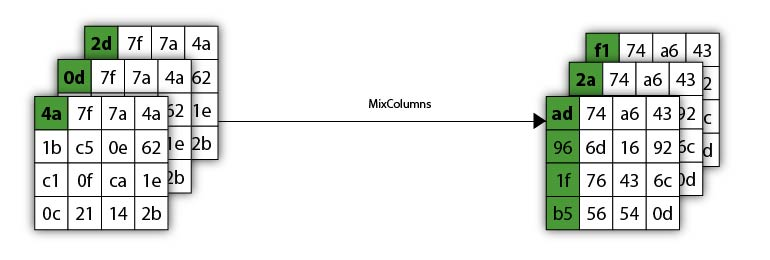
\includegraphics[width=0.8\textwidth]{figure/SQUARE-06.jpg}
\end{figure}
MixColumns 是 AES 中唯一的线性扩散层。它负责在列内进行线性组合,以列为单位,每一列左乘一个矩阵。将输列混合运算的状态矩阵的每一列的4个字节
以列向量表示,记为
\[ x = (x_0,x_1,x_2,x_3)^T  \]
输出的列向量记为
\[ y = (y_0,y_1,y_2,y_3)^T  \]
具体运算规则如下:
\begin{equation*}
\begin{bmatrix}
y_0 \\
y_1 \\
y_2 \\
y_3
\end{bmatrix} = 
\begin{bmatrix}
02 & 03 & 01 & 01 \\
01 & 02 & 03 & 01 \\
01 & 01 & 02 & 03 \\
03 & 01 & 01 & 02
\end{bmatrix}
\begin{bmatrix}
x_0 \\
x_1 \\
x_2 \\
x_3
\end{bmatrix} = 
\begin{bmatrix}
2 \cdot x_0 + 3 \cdot x_1 + x_2 + x_3 \\
x_0 + 2 \cdot x_1 + 3 \cdot x_2 + x_3 \\
x_0 + x_1 + 2 \cdot x_2 + 3 \cdot x_3 \\
3 \cdot x_0 + x_1 + x_2 + 2 \cdot x_3
\end{bmatrix}
\end{equation*}
我们的输入是第一列的活跃字节\(x_0\)和其他列的常数字节。经过 MixColumns 后，第一列的输出将是所有输入字节的线性组合，只要包含\(x_0\)，都会变成活跃字节，因为当\(x_0\)遍历 \(0 \dots 255\) 时，输出也会完整遍历 \(0 \dots 255\)。因此，MixColumns 不会破坏活跃字节的性质，但它会将活跃字节的影响扩散到整列。
\subsubsection{第一轮结束结果}
\begin{figure}[H]
    \centering
    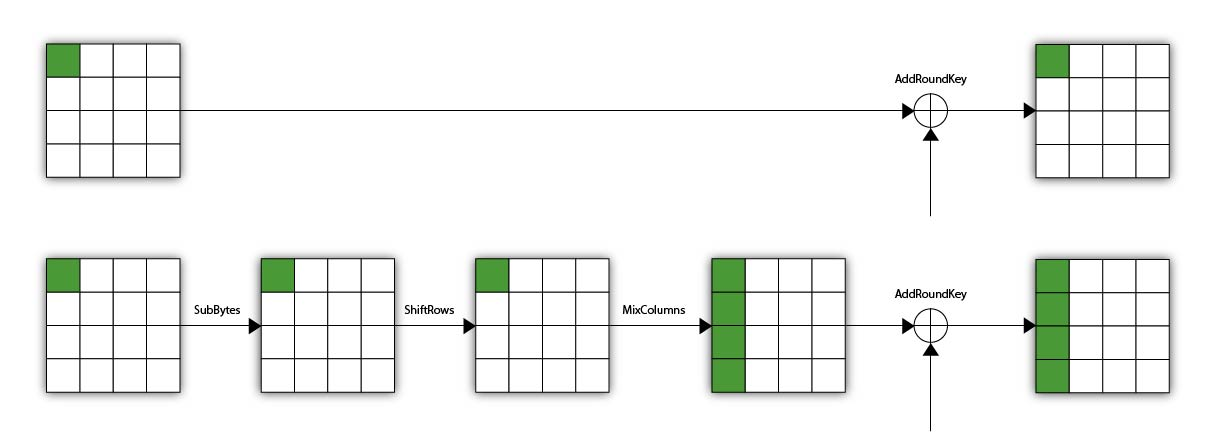
\includegraphics[width=0.8\textwidth]{figure/SQUARE-02.jpg}
\end{figure}
经过第一轮加密，我们得到了第一列都为活跃字节的状态。
\subsubsection{第二轮结束结果}
\begin{figure}[H]
    \centering
    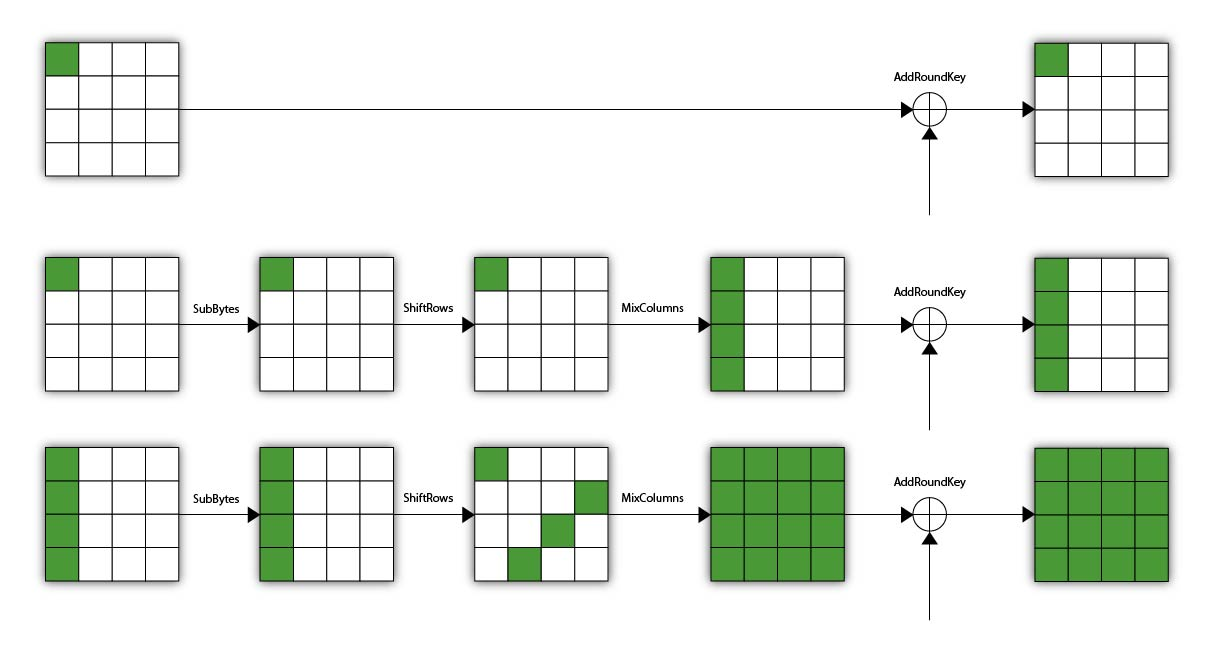
\includegraphics[width=0.8\textwidth]{figure/SQUARE-07.jpg}
\end{figure}
接下来进入第二轮，第二轮的 SubBytes 和 ShiftRows 不会改变活跃字节的数量，但ShiftRows会将第一列的活跃字节扩散到其他列，然后 MixColumns 会将这些活跃字节的影响扩散到整列。最终，在第二轮结束时，状态矩阵中的所有字节都变成了活跃字节。
\subsubsection{第三轮结束结果}
\begin{figure}[H]
    \centering
    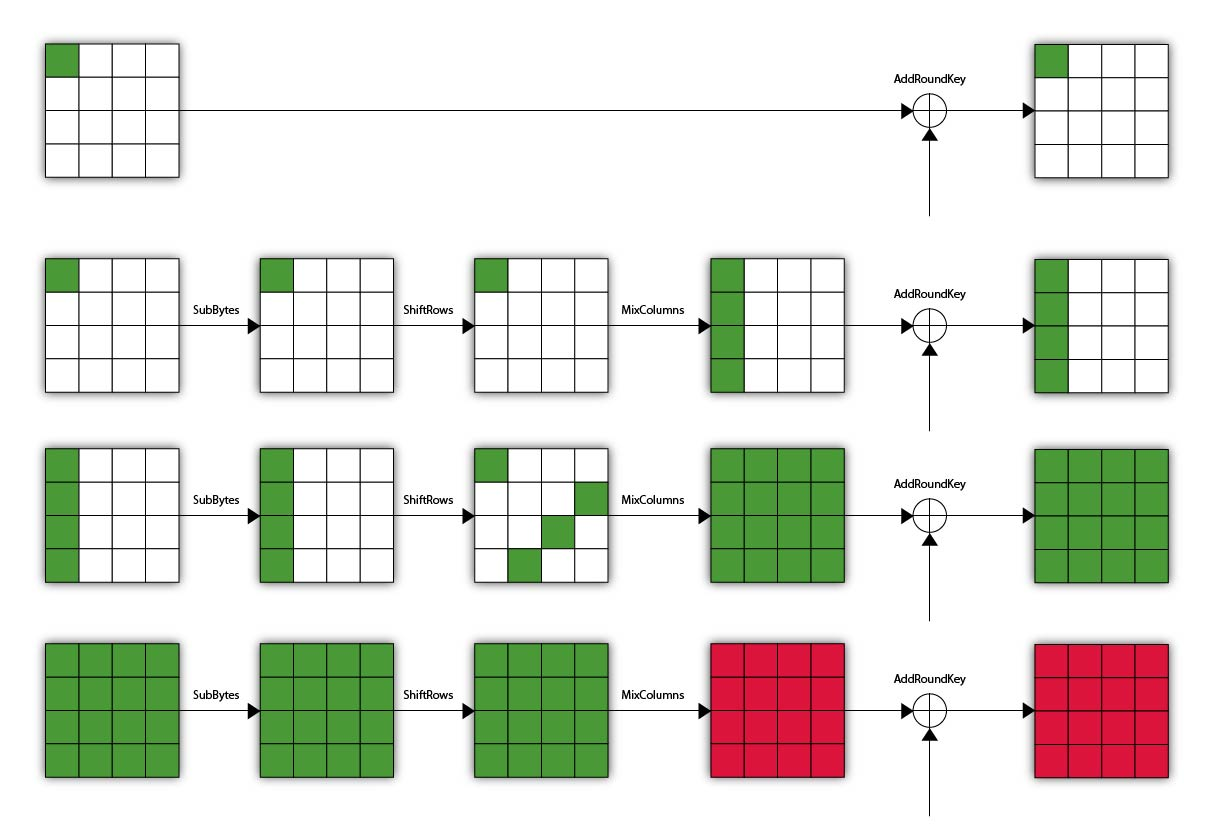
\includegraphics[width=0.8\textwidth]{figure/SQUARE-08.jpg}
\end{figure}
到了第三轮发生了变化，在MixColumns之后，活跃字节的线性组合，就不一定还是活跃字节了，因为\(y_i\)的取值范围可能被限制在一个子集内，导致无法遍历完整的 $0 \dots 255$。
这一点由实验结果验证了，比如\(y_0\)的取值大概只有160-170个
\begin{figure}[H]
    \centering
    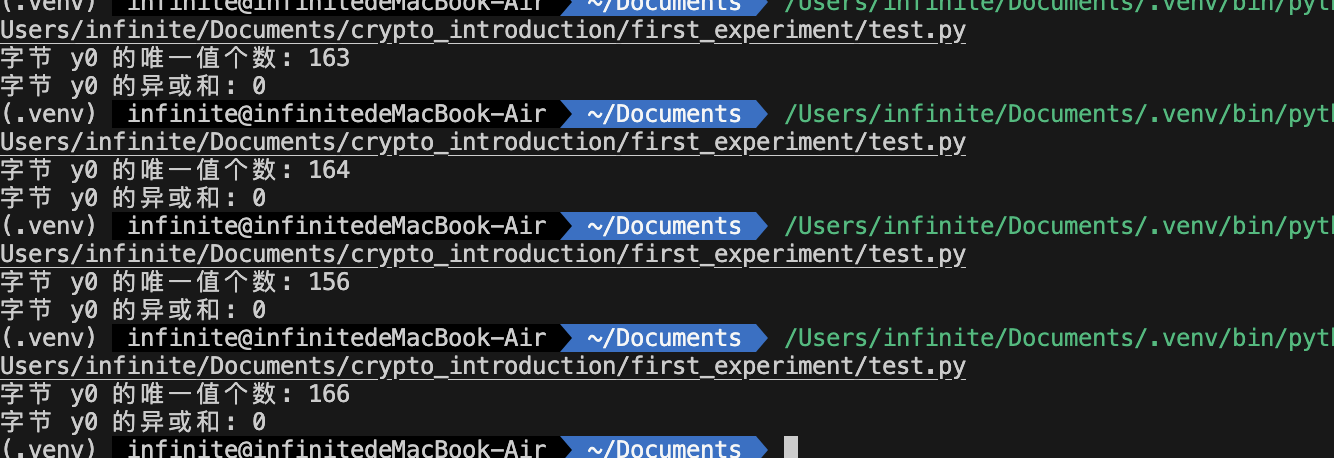
\includegraphics[width=0.8\textwidth]{figure/test.png}
\end{figure}
不过仍然满足异或和为0的性质

下面给出证明
\begin{equation*}
\begin{bmatrix}
y_0 \\
y_1 \\
y_2 \\
y_3
\end{bmatrix} = 
\begin{bmatrix}
02 & 03 & 01 & 01 \\
01 & 02 & 03 & 01 \\
01 & 01 & 02 & 03 \\
03 & 01 & 01 & 02
\end{bmatrix}
\begin{bmatrix}
x_{i,0} \\
x_{i,1} \\
x_{i,2} \\
x_{i,3}
\end{bmatrix} = 
\begin{bmatrix}
2 \cdot x_{i,0} + 3 \cdot x_{i,1} + x_{i,2} + x_{i,3} \\
x_{i,0} + 2 \cdot x_{i,1} + 3 \cdot x_{i,2} + x_{i,3} \\
x_{i,0} + x_{i,1} + 2 \cdot x_{i,2} + 3 \cdot x_{i,3} \\
3 \cdot x_{i,0} + x_{i,1} + x_{i,2} + 2 \cdot x_{i,3}
\end{bmatrix}
\end{equation*}
例如对于\(y_0\)，满足
\[
\bigoplus_{j=1}^{256} y_{0,j} = \bigoplus_{j=1}^{256} (2 \cdot x_{j,0} + 3 \cdot x_{j,1} + x_{j,2} + x_{j,3}) = 2\bigoplus_{j=1}^{256}  \cdot x_{j,0} \oplus 3\bigoplus_{j=1}^{256} \cdot x_{j,1} \oplus \bigoplus_{j=1}^{256} x_{j,2} \oplus \bigoplus_{j=1}^{256} x_{j,3} = 0
\]

所以在经过 3 轮 AES 加密后，其密文状态满足：
\begin{equation}
    \bigoplus_{i=1}^{256} C^{(i)} = 0
\end{equation}

\subsubsection{四轮的情况}
\begin{figure}[H]
    \centering
    \includegraphics[width=0.8\textwidth]{figure/Square-09.jpg}
\end{figure}
前面已经说明，经过三轮加密之后，密文异或和为0，但是在第四轮的 SubBytes 操作之后，这个性质就不再成立了。
不妨设经过SubBytes之后的\(y_0\)为\(z_0\)
\[
z_0 = S(y_0) = S(2 \cdot x_{i,0} + 3 \cdot x_{i,1} + x_{i,2} + x_{i,3})
\]
由于过S盒是一个非线性变换，所以不能像第三轮那样拆开来进行异或运算了，因此无法保证异或和为0
\begin{figure}[H]
    \centering
    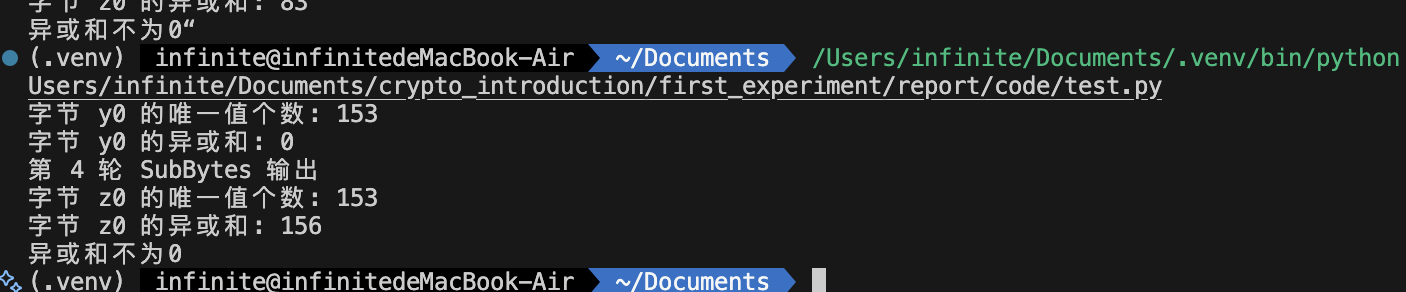
\includegraphics[width=0.8\textwidth]{figure/Round4.png}
\end{figure}


\subsubsection{删除 MixColumns 的影响}
实验发现，若删除 MixColumns，即使加密至 31 轮，平衡性依然保持。
这是因为没有 MixColumns 时，每个字节的变换仅由 S 盒复合组成。由于 S 盒是置换（Permutation），多个置换的复合依然是置换。如果输入遍历了 $0 \dots 255$，输出必然也完整遍历 $0 \dots 255$。
已知：
\begin{equation}
    \bigoplus_{i=0}^{255} i = 0
\end{equation}
故该现象在无扩散层时会永久保持。